\documentclass[conference]{IEEEtran}

\usepackage[utf8]{inputenc}
\usepackage{cite}
\usepackage{amsmath,amssymb,amsfonts}
\usepackage{graphicx}
\usepackage{xcolor}
\usepackage{tikz}
\usetikzlibrary{shapes.geometric, arrows.meta, positioning, fit, calc, backgrounds, patterns, circuits.logic.US, shapes.misc}
\usepackage{pgfplots}
\pgfplotsset{compat=1.17}
\usepackage{subcaption}
\usepackage{booktabs}

% Hardware component styles - REDUCED SIZES
\tikzset{
    register/.style={
        rectangle,
        draw=black,
        thick,
        minimum width=0.9cm,
        minimum height=0.6cm,
        fill=white,
        font=\tiny\ttfamily
    },
    mux/.style={
        trapezium,
        trapezium left angle=70,
        trapezium right angle=110,
        draw=black,
        thick,
        minimum width=0.6cm,
        minimum height=0.5cm,
        fill=white,
        font=\tiny
    },
    alu/.style={
        rectangle,
        draw=black,
        thick,
        minimum width=0.8cm,
        minimum height=0.9cm,
        fill=white,
        font=\tiny
    },
    memory/.style={
        rectangle,
        draw=black,
        very thick,
        minimum width=0.8cm,
        minimum height=1.2cm,
        fill=white,
        font=\tiny
    },
    wire/.style={
        draw=black,
        thick,
        -Stealth
    },
    bus/.style={
        draw=black,
        line width=1.2pt,
        -Stealth
    },
    controlwire/.style={
        draw=black,
        dashed,
        -Stealth
    },
    buswidth/.style={
        font=\tiny,
        fill=white,
        inner sep=0.5pt
    },
    logic/.style={
        rectangle,
        draw=black,
        thick,
        rounded corners=2pt,
        minimum width=0.6cm,
        minimum height=0.5cm,
        fill=gray!10,
        font=\tiny
    },
    sbox/.style={
        rectangle,
        draw=black,
        thick,
        minimum width=0.5cm,
        minimum height=0.5cm,
        fill=gray!20,
        font=\tiny
    }
}

\begin{document}

\title{AES-128 Hardware Architecture:\\RTL Implementation on FPGA}

\author{\IEEEauthorblockN{Hardware Implementation}
\IEEEauthorblockA{Register-Transfer Level Design}}

\maketitle

%==============================================================================
% Figure 1: Complete Datapath Architecture - SPLIT INTO TWO PARTS
%==============================================================================
\begin{figure*}[!t]
\centering
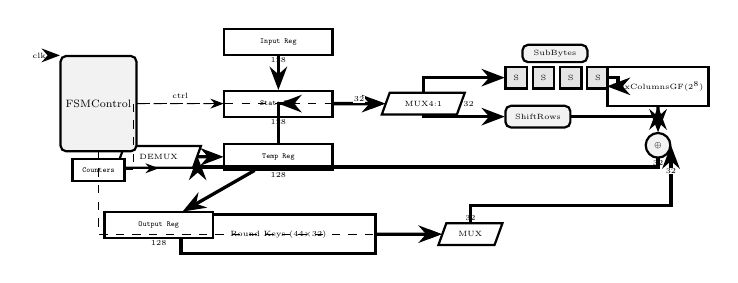
\begin{tikzpicture}[node distance=0.5cm and 0.7cm, scale=0.55, transform shape]

% Input Register
\node[register, minimum width=2.5cm] (input_reg) {Input Reg};
\node[buswidth] at (input_reg.south) [below=0.02cm] {128};

% State Register
\node[register, minimum width=2.5cm, below=0.8cm of input_reg] (state_reg) {State Reg};
\node[buswidth] at (state_reg.south) [below=0.02cm] {128};

% Column Multiplexer
\node[mux, right=1.2cm of state_reg, minimum width=1.2cm] (col_mux) {MUX\\4:1};
\node[buswidth] at (col_mux.east) [right=0.02cm] {32};

% S-boxes (32-bit processing)
\node[sbox, right=1cm of col_mux, yshift=0.6cm] (sbox0) {S};
\node[sbox, right=0.1cm of sbox0] (sbox1) {S};
\node[sbox, right=0.1cm of sbox1] (sbox2) {S};
\node[sbox, right=0.1cm of sbox2] (sbox3) {S};
\node[logic, above=0.08cm of sbox1.north east, minimum width=1.5cm, minimum height=0.4cm] (sb_label) {\tiny SubBytes};

% ShiftRows
\node[logic, right=1cm of col_mux, yshift=-0.3cm, minimum width=1.5cm, minimum height=0.5cm] (shiftrows) {\tiny ShiftRows};

% MixColumns
\node[alu, right=1.2cm of sbox1, yshift=-0.2cm, minimum width=1.4cm, minimum height=0.9cm] (mixcol) {\tiny MixColumns\\[-0.05cm]\tiny GF($2^8$)};

% XOR for AddRoundKey
\node[logic, circle, minimum size=0.4cm, below=0.6cm of mixcol] (xor_array) {$\oplus$};
\node[buswidth] at (xor_array.south) [below=0.02cm] {32};

% Temp Register
\node[register, minimum width=2.5cm, below=0.6cm of state_reg] (temp_reg) {Temp Reg};
\node[buswidth] at (temp_reg.south) [below=0.02cm] {128};

% Demux
\node[mux, left=0.6cm of temp_reg, minimum width=1.2cm, shape border rotate=180] (col_demux) {DEMUX};

% Key Storage
\node[memory, below=1cm of temp_reg, minimum width=4.5cm, minimum height=0.9cm] (key_storage) {\tiny Round Keys (44$\times$32)};

% Round Key Mux
\node[mux, right=1.5cm of key_storage, minimum width=1cm] (rkey_mux) {MUX};
\node[buswidth] at (rkey_mux.north) [above=0.02cm] {32};

% Output Register
\node[register, minimum width=2.5cm, below=1cm of col_demux] (output_reg) {Output Reg};
\node[buswidth] at (output_reg.south) [below=0.02cm] {128};

% FSM Control
\node[logic, left=2cm of state_reg, minimum width=1.5cm, minimum height=2.2cm] (fsm) {\scriptsize FSM\\[-0.05cm]\scriptsize Control};
\node[register, below=0.15cm of fsm, minimum width=1.2cm, minimum height=0.5cm] (counters) {\tiny Counters};

% Connections
\draw[bus] (input_reg) -- (state_reg);
\draw[bus] (state_reg) -- node[buswidth, above] {32} (col_mux);
\draw[bus] (col_mux.north) |- (sbox0.west);
\draw[bus] (sbox3.east) -- ++(0.2,0) |- (mixcol.west);
\draw[bus] (col_mux.south) |- (shiftrows.west);
\draw[bus] (shiftrows.east) -| (mixcol.south);
\draw[bus] (mixcol) -- (xor_array);
\draw[bus] (xor_array.south) -- ++(0,-0.2) -| (col_demux.east);
\draw[bus] (col_demux) -- (temp_reg);
\draw[bus] (temp_reg) |- (state_reg);
\draw[bus] (temp_reg) -- (output_reg);

% Key connections
\draw[bus] (key_storage) -- (rkey_mux);
\draw[bus] (rkey_mux.north) -- ++(0,0.4) -| node[buswidth, near end, above] {32} (xor_array.east);

% Control signals
\draw[controlwire] (fsm) -- node[above, font=\tiny] {ctrl} (state_reg);
\draw[controlwire] (counters.east) -- ++(0.2,0) |- (col_mux.west);
\draw[controlwire] (counters.east) -- ++(0.3,0) |- (col_demux.south);
\draw[controlwire] (fsm) |- (rkey_mux.west);

% Clock
\node[font=\tiny, left=0.2cm of fsm.north west] (clk) {clk};
\draw[wire] (clk) -- (fsm.north west);

\end{tikzpicture}
\caption{Complete AES datapath showing register-transfer level implementation with 32-bit column-wise processing, parallel S-boxes, and control signals.}
\label{fig:datapath}
\end{figure*}

\clearpage

%==============================================================================
% Figure 2: Pipeline Comparison
%==============================================================================
\begin{figure*}[!t]
\centering
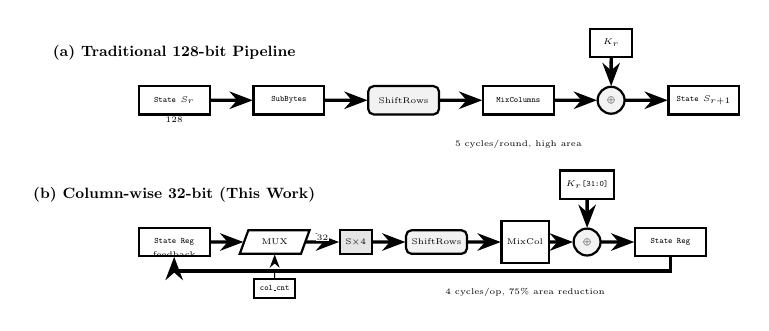
\begin{tikzpicture}[node distance=0.5cm and 0.9cm, scale=0.6, transform shape]

% Top: Traditional pipeline
\node[font=\small\bfseries] at (0,3.5) {(a) Traditional 128-bit Pipeline};

\node[register, minimum width=1.5cm] (s0) at (0,2.5) {State $S_r$};
\node[register, minimum width=1.5cm, right=of s0] (sb) {SubBytes};
\node[logic, right=of sb, minimum width=1.5cm, minimum height=0.6cm] (sr) {ShiftRows};
\node[register, minimum width=1.5cm, right=of sr] (mc) {MixColumns};
\node[logic, circle, minimum size=0.5cm, right=of mc] (xor) {$\oplus$};
\node[register, minimum width=1.5cm, right=of xor] (s1) {State $S_{r+1}$};

\node[register, above=0.6cm of xor] (rkey) {$K_r$};
\draw[bus] (rkey) -- (xor);

\draw[bus] (s0) -- (sb);
\draw[bus] (sb) -- (sr);
\draw[bus] (sr) -- (mc);
\draw[bus] (mc) -- (xor);
\draw[bus] (xor) -- (s1);

\node[buswidth] at (s0.south) [below=0.02cm] {128};
\node[font=\tiny, below=0.4cm of mc] {5 cycles/round, high area};

% Bottom: Column-wise
\node[font=\small\bfseries] at (0,0.5) {(b) Column-wise 32-bit (This Work)};

\node[register, minimum width=1.5cm] (cs0) at (0,-0.5) {State Reg};
\node[mux, right=0.7cm of cs0] (cmux) {MUX};
\node[sbox, right=0.7cm of cmux] (csb) {S$\times$4};
\node[logic, right=0.7cm of csb, minimum width=1.2cm] (csr) {\tiny ShiftRows};
\node[alu, right=0.7cm of csr, minimum width=1cm] (cmc) {\tiny MixCol};
\node[logic, circle, minimum size=0.4cm, right=0.5cm of cmc] (cxor) {$\oplus$};
\node[register, minimum width=1.5cm, right=0.7cm of cxor] (cs1) {State Reg};

\node[register, above=0.6cm of cxor] (crkey) {$K_r$[31:0]};
\draw[bus] (crkey) -- (cxor);

\draw[bus] (cs0) -- (cmux);
\draw[bus] (cmux) -- node[buswidth, above] {32} (csb);
\draw[bus] (csb) -- (csr);
\draw[bus] (csr) -- (cmc);
\draw[bus] (cmc) -- (cxor);
\draw[bus] (cxor) -- (cs1);
\draw[bus] (cs1.south) -- ++(0,-0.3) -| node[near end, above, font=\tiny] {feedback} (cs0.south);

\node[register, below=0.5cm of cmux, minimum width=0.8cm, minimum height=0.4cm] (ccnt) {\tiny col\_cnt};
\draw[controlwire] (ccnt) -- (cmux);

\node[font=\tiny, below=0.4cm of cmc] {4 cycles/op, 75\% area reduction};

\end{tikzpicture}
\caption{Pipeline architecture comparison: (a) traditional 128-bit full-width pipeline vs (b) column-wise 32-bit sequential processing with resource savings.}
\label{fig:pipeline}
\end{figure*}

\clearpage

%==============================================================================
% Figure 3: Key Expansion Hardware
%==============================================================================
\begin{figure}[!t]
\centering
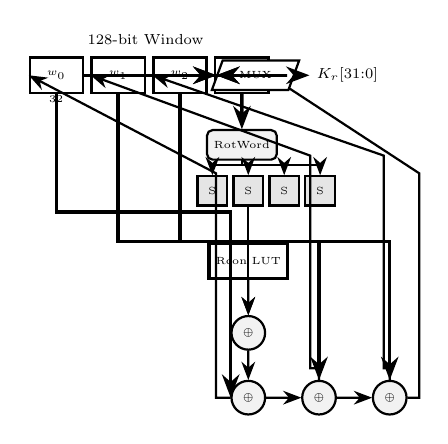
\begin{tikzpicture}[node distance=0.5cm and 0.6cm, scale=0.75, transform shape]

% Key window registers
\node[register, minimum width=0.9cm, minimum height=0.6cm] (w0) {$w_0$};
\node[register, minimum width=0.9cm, minimum height=0.6cm, right=0.12cm of w0] (w1) {$w_1$};
\node[register, minimum width=0.9cm, minimum height=0.6cm, right=0.12cm of w1] (w2) {$w_2$};
\node[register, minimum width=0.9cm, minimum height=0.6cm, right=0.12cm of w2] (w3) {$w_3$};

\node[font=\scriptsize, above=0.08cm of w1.north east] {128-bit Window};
\node[buswidth] at (w0.south) [below=0.01cm] {32};

% RotWord
\node[logic, below=0.6cm of w3, minimum width=0.9cm] (rotword) {\tiny RotWord};
\draw[bus] (w3) -- (rotword);

% S-boxes
\node[sbox, below=0.25cm of rotword, xshift=-0.5cm] (ks0) {S};
\node[sbox, right=0.08cm of ks0] (ks1) {S};
\node[sbox, right=0.08cm of ks1] (ks2) {S};
\node[sbox, right=0.08cm of ks2] (ks3) {S};

\draw[wire] (rotword.south) -- ++(0,-0.08) -| (ks0.north);
\draw[wire] (rotword.south) -- ++(0,-0.08) -| (ks1.north);
\draw[wire] (rotword.south) -- ++(0,-0.08) -| (ks2.north);
\draw[wire] (rotword.south) -- ++(0,-0.08) -| (ks3.north);

% Rcon
\node[memory, below=0.6cm of ks1, minimum width=1.2cm, minimum height=0.6cm] (rcon) {\tiny Rcon LUT};

% XOR chain
\node[logic, circle, minimum size=0.35cm, below=0.6cm of rcon] (xor1) {$\oplus$};
\node[logic, circle, minimum size=0.35cm, below=0.5cm of xor1] (xor2) {$\oplus$};
\node[logic, circle, minimum size=0.35cm, right=0.6cm of xor2] (xor3) {$\oplus$};
\node[logic, circle, minimum size=0.35cm, right=0.6cm of xor3] (xor4) {$\oplus$};

\draw[wire] (ks1.south) -- ++(0,-0.15) -| (xor1.north);
\draw[wire] (rcon) -- (xor1);
\draw[bus] (w0.south) -- ++(0,-2) -| (xor2.west);
\draw[wire] (xor1) -- (xor2);
\draw[wire] (xor2) -- (xor3);
\draw[bus] (w1.south) -- ++(0,-2.5) -| (xor3.north);
\draw[bus] (w2.south) -- ++(0,-2.5) -| (xor4.north);
\draw[wire] (xor3) -- (xor4);

% Feedback
\draw[wire] (xor2.west) -- ++(-0.25,0) -- ++(0,3.8) -- (w0.west);
\draw[wire] (xor3.north) -- ++(0,0.2) -- ++(-0.15,0) -- ++(0,3.6) -- (w1.west);
\draw[wire] (xor4.north) -- ++(0,0.2) -- ++(-0.1,0) -- ++(0,3.6) -- (w2.west);
\draw[wire] (xor4.east) -- ++(0.2,0) -- ++(0,3.8) -- (w3.east);

% Output mux
\node[mux, right=1.2cm of w1, minimum width=0.8cm] (outmux) {MUX};
\draw[bus] (w0.east) -- ++(0.15,0) |- (outmux.west);
\draw[bus] (w1.east) -- ++(0.2,0) |- (outmux.west);
\draw[bus] (w2.east) -- ++(0.25,0) |- (outmux.west);
\draw[bus] (w3.east) -- ++(0.3,0) |- (outmux.west);

\node[right=0.25cm of outmux, font=\scriptsize] (keyout) {$K_r$[31:0]};
\draw[bus] (outmux) -- (keyout);

\end{tikzpicture}
\caption{On-the-fly key expansion hardware with 4-word register window, achieving 90\% memory reduction vs. storing all 44 words.}
\label{fig:keyexp}
\end{figure}

\clearpage

%==============================================================================
% Figure 4: SubBytes Implementation
%==============================================================================
\begin{figure}[!t]
\centering
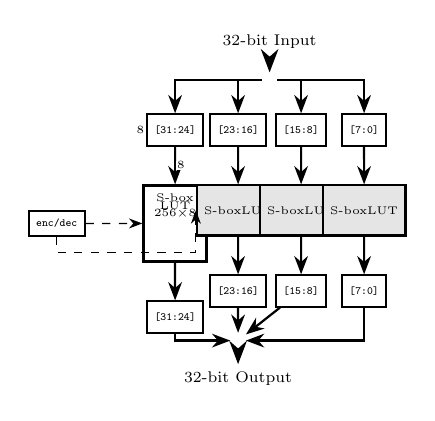
\begin{tikzpicture}[node distance=0.5cm and 0.6cm, scale=0.8, transform shape]

% Input
\node[font=\scriptsize] (input) {32-bit Input};
\node[below=0.25cm of input] (split) {};

% Split into bytes
\node[register, below=0.4cm of split, xshift=-1.5cm, minimum width=0.7cm, minimum height=0.5cm] (b0) {[31:24]};
\node[register, below=0.4cm of split, xshift=-0.5cm, minimum width=0.7cm, minimum height=0.5cm] (b1) {[23:16]};
\node[register, below=0.4cm of split, xshift=0.5cm, minimum width=0.7cm, minimum height=0.5cm] (b2) {[15:8]};
\node[register, below=0.4cm of split, xshift=1.5cm, minimum width=0.7cm, minimum height=0.5cm] (b3) {[7:0]};

\draw[bus] (input) -- (split);
\draw[wire] (split) -| (b0);
\draw[wire] (split) -| (b1);
\draw[wire] (split) -| (b2);
\draw[wire] (split) -| (b3);

\node[buswidth] at (b0.west) [left=0.01cm] {8};

% S-boxes
\node[memory, below=0.6cm of b0, minimum width=1cm, minimum height=1.2cm] (sbox0) {};
\node[font=\tiny, below=0.03cm of sbox0.north] {S-box};
\node[font=\tiny, below=0.15cm of sbox0.north] {LUT};
\node[font=\tiny, below=0.27cm of sbox0.north] {256$\times$8};

\node[sbox, below=0.6cm of b1, minimum width=0.8cm, minimum height=0.8cm] (sbox1) {\tiny S-box\\[-0.05cm]\tiny LUT};
\node[sbox, below=0.6cm of b2, minimum width=0.8cm, minimum height=0.8cm] (sbox2) {\tiny S-box\\[-0.05cm]\tiny LUT};
\node[sbox, below=0.6cm of b3, minimum width=0.8cm, minimum height=0.8cm] (sbox3) {\tiny S-box\\[-0.05cm]\tiny LUT};

\draw[wire] (b0) -- node[buswidth, right] {8} (sbox0);
\draw[wire] (b1) -- (sbox1);
\draw[wire] (b2) -- (sbox2);
\draw[wire] (b3) -- (sbox3);

% Output bytes
\node[register, below=0.6cm of sbox0, minimum width=0.7cm, minimum height=0.5cm] (ob0) {[31:24]};
\node[register, below=0.6cm of sbox1, minimum width=0.7cm, minimum height=0.5cm] (ob1) {[23:16]};
\node[register, below=0.6cm of sbox2, minimum width=0.7cm, minimum height=0.5cm] (ob2) {[15:8]};
\node[register, below=0.6cm of sbox3, minimum width=0.7cm, minimum height=0.5cm] (ob3) {[7:0]};

\draw[wire] (sbox0) -- (ob0);
\draw[wire] (sbox1) -- (ob1);
\draw[wire] (sbox2) -- (ob2);
\draw[wire] (sbox3) -- (ob3);

% Merge
\node[below=0.4cm of ob1] (merge) {};
\node[font=\scriptsize, below=0.25cm of merge] (output) {32-bit Output};

\draw[wire] (ob0) |- (merge);
\draw[wire] (ob1) -- (merge);
\draw[wire] (ob2) -- (merge);
\draw[wire] (ob3) |- (merge);
\draw[bus] (merge) -- (output);

% Control
\node[register, left=0.9cm of sbox0, minimum width=0.7cm, minimum height=0.4cm] (mode) {\tiny enc/dec};
\draw[controlwire] (mode) -- (sbox0.west);
\draw[controlwire] (mode.south) -- ++(0,-0.25) -| (sbox1.west);

\end{tikzpicture}
\caption{SubBytes hardware with four parallel 256$\times$8-bit S-box LUTs for 32-bit processing. Control selects forward or inverse S-box.}
\label{fig:subbytes}
\end{figure}

\clearpage

%==============================================================================
% Figure 5: MixColumns Hardware
%==============================================================================
\begin{figure}[!t]
\centering
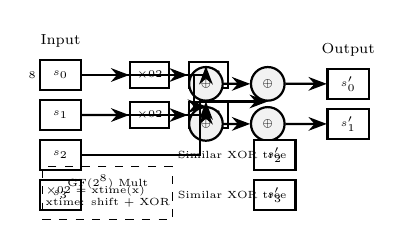
\begin{tikzpicture}[node distance=0.4cm and 0.5cm, scale=0.75, transform shape]

% Input bytes
\node[register, minimum width=0.7cm, minimum height=0.5cm] (s0) {$s_0$};
\node[register, minimum width=0.7cm, minimum height=0.5cm, below=0.15cm of s0] (s1) {$s_1$};
\node[register, minimum width=0.7cm, minimum height=0.5cm, below=0.15cm of s1] (s2) {$s_2$};
\node[register, minimum width=0.7cm, minimum height=0.5cm, below=0.15cm of s2] (s3) {$s_3$};

\node[font=\scriptsize, above=0.08cm of s0] {Input};
\node[buswidth, font=\tiny, left=0.03cm of s0.west] {8};

% GF multipliers
\node[alu, right=0.8cm of s0, minimum width=0.6cm, minimum height=0.45cm] (m02_0) {\tiny$\times$02};
\node[alu, right=0.3cm of m02_0, minimum width=0.6cm, minimum height=0.45cm] (m03_0) {\tiny$\times$03};

\node[alu, right=0.8cm of s1, minimum width=0.6cm, minimum height=0.45cm] (m02_1) {\tiny$\times$02};
\node[alu, right=0.3cm of m02_1, minimum width=0.6cm, minimum height=0.45cm] (m03_1) {\tiny$\times$03};

\draw[wire] (s0) -- (m02_0);
\draw[wire] (s0.east) -- ++(0.25,0) |- (m03_0.west);
\draw[wire] (s1) -- (m02_1);
\draw[wire] (s1.east) -- ++(0.25,0) |- (m03_1.west);

% XOR trees (simplified for space)
\node[logic, circle, minimum size=0.3cm, right=1.8cm of s0, yshift=-0.15cm] (xor0) {$\oplus$};
\node[logic, circle, minimum size=0.3cm, right=0.45cm of xor0] (xor0_2) {$\oplus$};

\node[logic, circle, minimum size=0.3cm, right=1.8cm of s1, yshift=-0.15cm] (xor1) {$\oplus$};
\node[logic, circle, minimum size=0.3cm, right=0.45cm of xor1] (xor1_2) {$\oplus$};

\draw[wire] (m02_0) -| (xor0);
\draw[wire] (m03_1) -| (xor0);
\draw[wire] (xor0) -- (xor0_2);
\draw[wire] (s2.east) -- ++(2,0) |- (xor0_2.south);

\draw[wire] (m02_1) -| (xor1);
\draw[wire] (s0.east) -- ++(1.9,0) |- (xor1.north);
\draw[wire] (xor1) -- (xor1_2);

% Output
\node[register, right=0.7cm of xor0_2, minimum width=0.7cm, minimum height=0.5cm] (out0) {$s_0'$};
\node[register, right=0.7cm of xor1_2, minimum width=0.7cm, minimum height=0.5cm] (out1) {$s_1'$};
\node[register, right=2.9cm of s2, minimum width=0.7cm, minimum height=0.5cm] (out2) {$s_2'$};
\node[register, right=2.9cm of s3, minimum width=0.7cm, minimum height=0.5cm] (out3) {$s_3'$};

\draw[wire] (xor0_2) -- (out0);
\draw[wire] (xor1_2) -- (out1);

\node[font=\scriptsize, above=0.08cm of out0] {Output};

% Similar annotation for s2, s3
\node[font=\tiny, right=1.5cm of s2] {Similar XOR tree};
\node[font=\tiny, right=1.5cm of s3] {Similar XOR tree};

% GF multiplier detail
\node[draw, dashed, below=0.6cm of s1, minimum width=2.2cm, minimum height=0.9cm, xshift=0.8cm] (gf) {};
\node[font=\tiny, below=0.03cm of gf.north] {GF($2^8$) Mult};
\node[font=\tiny, below=0.2cm of gf.north, align=left] {
$\times$02 = xtime(x)\\
xtime: shift + XOR
};

\end{tikzpicture}
\caption{MixColumns hardware with GF($2^8$) multipliers and XOR trees implementing matrix multiplication for one column.}
\label{fig:mixcol}
\end{figure}

\clearpage

%==============================================================================
% Figure 6: Control FSM
%==============================================================================
\begin{figure}[!t]
\centering
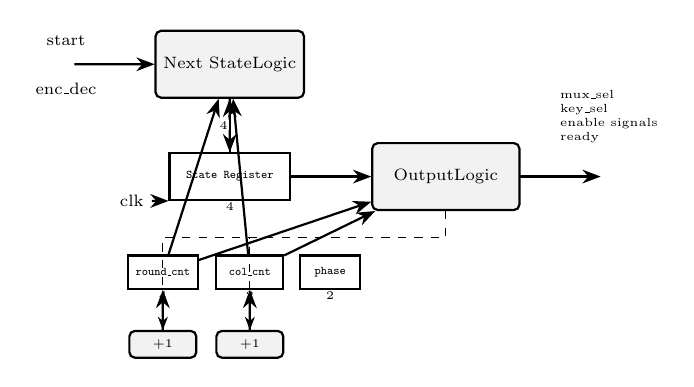
\begin{tikzpicture}[node distance=0.6cm and 0.8cm, scale=0.85, transform shape]

% State register
\node[register, minimum width=1.8cm, minimum height=0.7cm] (state_reg) {State Register};
\node[buswidth] at (state_reg.south) [below=0.01cm] {4};

% Next state logic
\node[logic, above=0.8cm of state_reg, minimum width=2.2cm, minimum height=1cm] (nsl) {\scriptsize Next State\\[-0.05cm]\scriptsize Logic};

% Output logic
\node[logic, right=1.2cm of state_reg, minimum width=2.2cm, minimum height=1cm] (output) {\scriptsize Output\\[-0.05cm]\scriptsize Logic};

% Counters
\node[register, below=0.8cm of state_reg, xshift=-1cm, minimum width=1cm, minimum height=0.5cm] (round) {\tiny round\_cnt};
\node[buswidth] at (round.south) [below=0.01cm] {4};

\node[register, below=0.8cm of state_reg, xshift=0.3cm, minimum width=1cm, minimum height=0.5cm] (col) {\tiny col\_cnt};
\node[buswidth] at (col.south) [below=0.01cm] {2};

\node[register, below=0.8cm of state_reg, xshift=1.5cm, minimum width=0.9cm, minimum height=0.5cm] (phase) {\tiny phase};
\node[buswidth] at (phase.south) [below=0.01cm] {2};

% Increment logic
\node[logic, below=0.6cm of round, minimum width=1cm, minimum height=0.4cm] (inc1) {\tiny +1};
\node[logic, below=0.6cm of col, minimum width=1cm, minimum height=0.4cm] (inc2) {\tiny +1};

% Inputs
\node[left=1.2cm of nsl] (inputs) {};
\node[font=\scriptsize, above=0.03cm of inputs] {start};
\node[font=\scriptsize, below=0.03cm of inputs] {enc\_dec};

% Outputs
\node[right=1.2cm of output] (outputs) {};
\node[font=\tiny, above=0.25cm of outputs, align=left] {
mux\_sel\\
key\_sel\\
enable signals\\
ready
};

% Control flow
\draw[wire] (state_reg) -- (nsl);
\draw[wire] (nsl) -- node[buswidth, left] {4} (state_reg);
\draw[wire] (state_reg) -- (output);
\draw[wire] (output) -- (outputs);
\draw[wire] (inputs) -- (nsl);

% Counter connections
\draw[wire] (round) -- (nsl);
\draw[wire] (col) -- (nsl);
\draw[wire] (round) -- (output);
\draw[wire] (col) -- (output);

\draw[controlwire] (output.south) -- ++(0,-0.4) -| (inc1.north);
\draw[controlwire] (output.south) -- ++(0,-0.4) -| (inc2.north);
\draw[wire] (inc1) -- (round);
\draw[wire] (inc2) -- (col);

% Clock
\node[font=\scriptsize, left=0.25cm of state_reg.south west] (clk) {clk};
\draw[wire] (clk) -- (state_reg.south west);

\end{tikzpicture}
\caption{Control FSM hardware showing state register, next-state logic, output logic, and round/column counters with increment logic.}
\label{fig:fsm}
\end{figure}

\end{document}
